\documentclass{article}
\usepackage{graphicx} % Required for inserting images
% Change page dimensions
\usepackage[margin=1in]{geometry}
\usepackage{amsmath}
\usepackage{subcaption} % in preamble

\title{Time Impact to Sentiment Analysis}
\author{Leon King}
\date{August 2025}

\begin{document}

\maketitle

\section{Introduction}
We aim to investigate how the ratings of wine reviews vary by year and sentiment scores. 

\section{Background}
After we run the AMIC model on the wine review dataset and get the predicted sentiment scores for each wine review, we want to use these sentiment scores to study the changes in rating scores by year. AMIC is a model that integrates self-attention language models with traditional logistics regression. 

\section{Dataset}
I used the part of the new dataset that contains a valid review year. The total number of reviews is 13,696.
\begin{figure}[!ht]
    \centering
    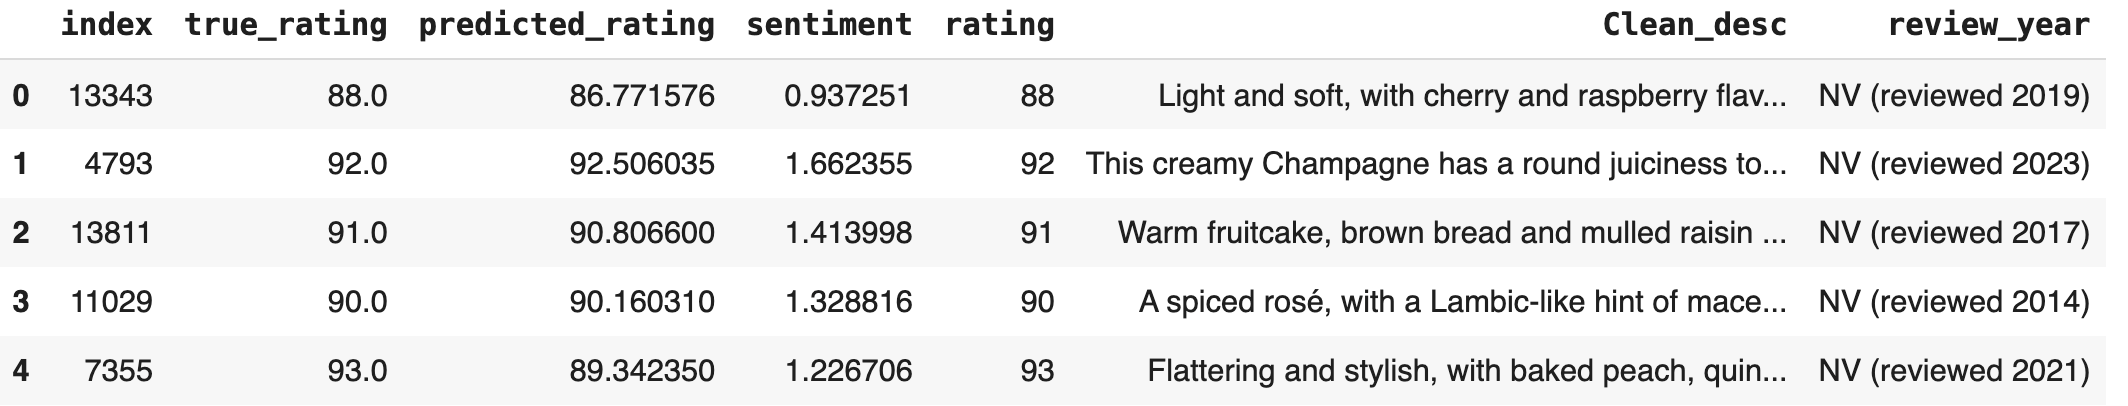
\includegraphics[width=1.0\linewidth]{wine_data.png}
    \caption{Wine Review Data Snap}
    \label{fig:placeholder}
\end{figure}

The rating score distribution is roughly 60-100, and the sentiment range is from 0 to 2.5.
\begin{figure}[!ht]
    \centering
    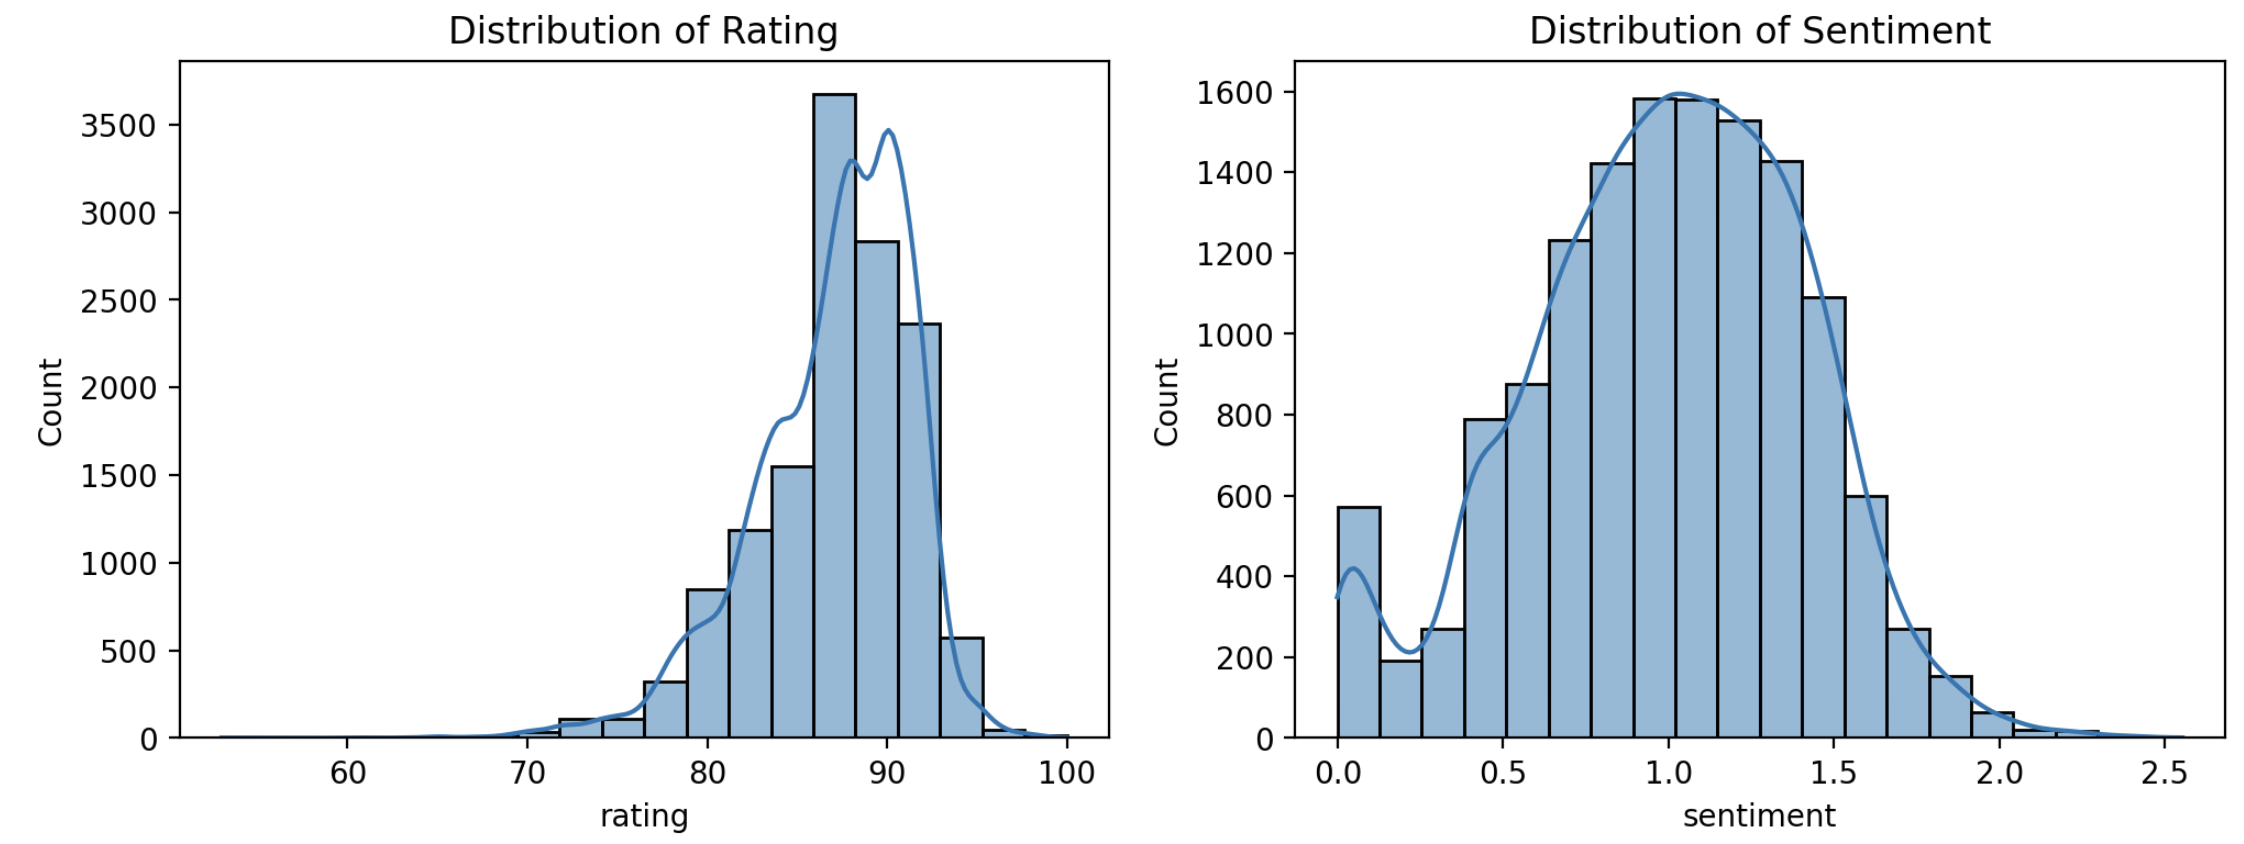
\includegraphics[width=0.75\linewidth]{distribution.png}
    \caption{Distribution of Rating and Sentiment}
    \label{fig:placeholder}
\end{figure}

The review year is from 1985 to 2025. The most reviews happened in 2015.
\begin{figure}[!ht]
    \centering
    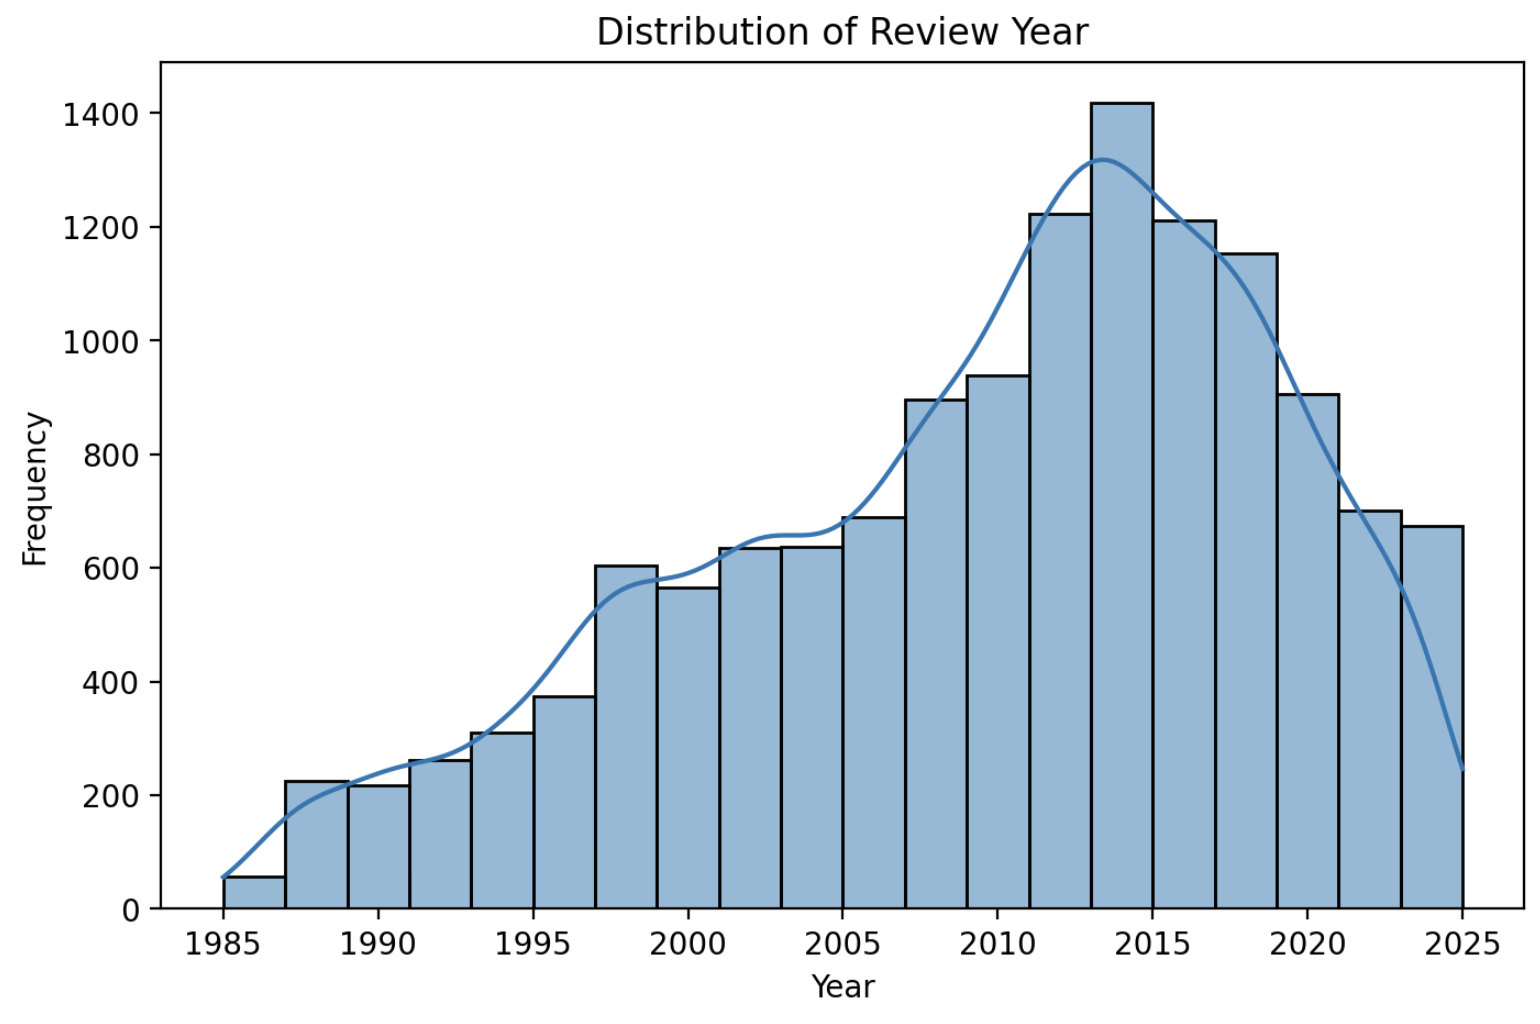
\includegraphics[width=0.5\linewidth]{review_year.png}
    \caption{Enter Caption}
    \label{fig:placeholder}
\end{figure}

\section{Simple Linear Regression}
The first step I took was to do a simple linear regression on rating by the variables: year, sentiment. I consider the year as a continuous variable. The summary of the regression is attached as follows. The adjusted R-squared is 0.796. 79.6\% of rating variability is explained by year and sentiment. The remaining 20\% rating variability is explained by factors that don't appear in the model. However, 79.6\% still shows the relationship between rating and the two variables is strong. The p-values of two variables are statistically significant, especially the variable sentiment, which makes sense that sentiments are AMIC model outcomes.  

$$\text{rating} = \beta_0 + \beta_1 \cdot \text{year} + \beta_2 \cdot \text{sentiment} + \varepsilon$$
$$E(\text{rating}) = 27.3 + 0.02 \cdot \text{year} + 9.03 \cdot \text{sentiment}$$
\begin{figure}[!ht]
    \centering
    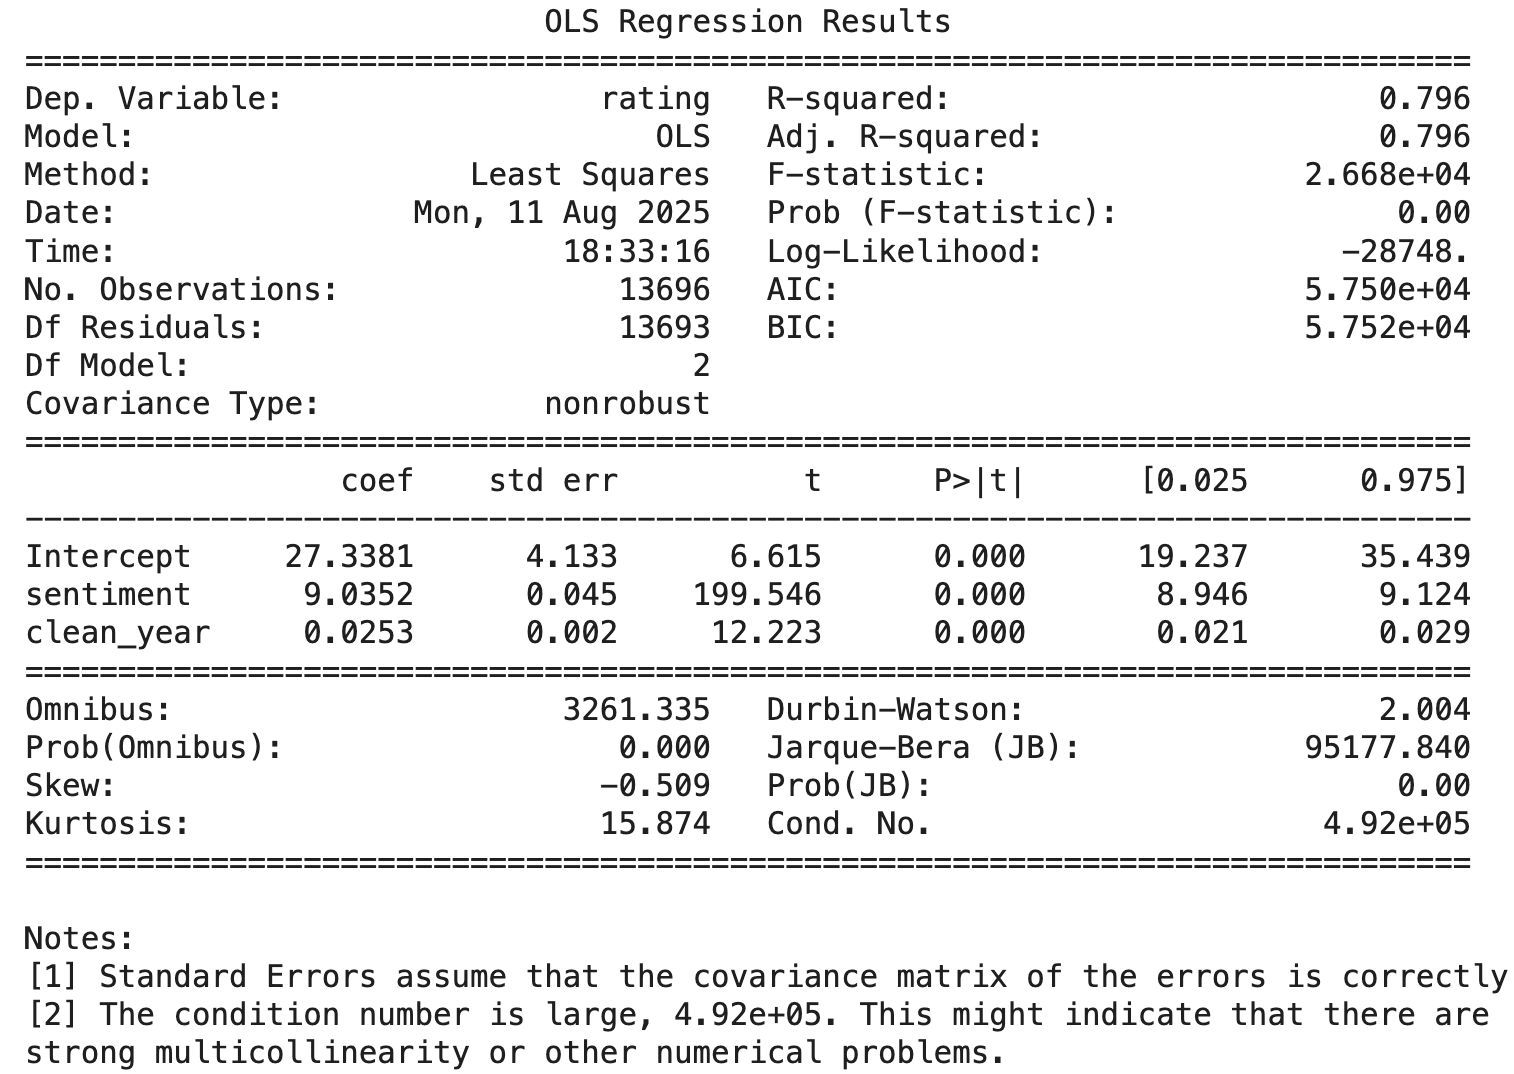
\includegraphics[width=0.5\linewidth]{linear_regression.png}
    \caption{Summary of Linear Regression}
    \label{fig:placeholder}
\end{figure}

The following plot shows the relationship between sentiment on the x-axis and rating on the y-axis. It shows a robust positive relationship, reinforcing our earlier simple linear regression. As we can observe, the variation of rating becomes less when the sentiment score is higher. 

The following graph is the residuals versus sentiment from this linear regression. As we can observe, the residuals are evenly scattered across the solid zero line and majority of residuals fall within the absolute value 10. The residuals are much smaller when the sentiment scores are higher, which confirms our previous conclusion about the relationship between rating and sentiment.
\begin{figure}[!ht]
    \centering
    % First subfigure
    \begin{subfigure}[b]{0.45\linewidth}
        \centering
        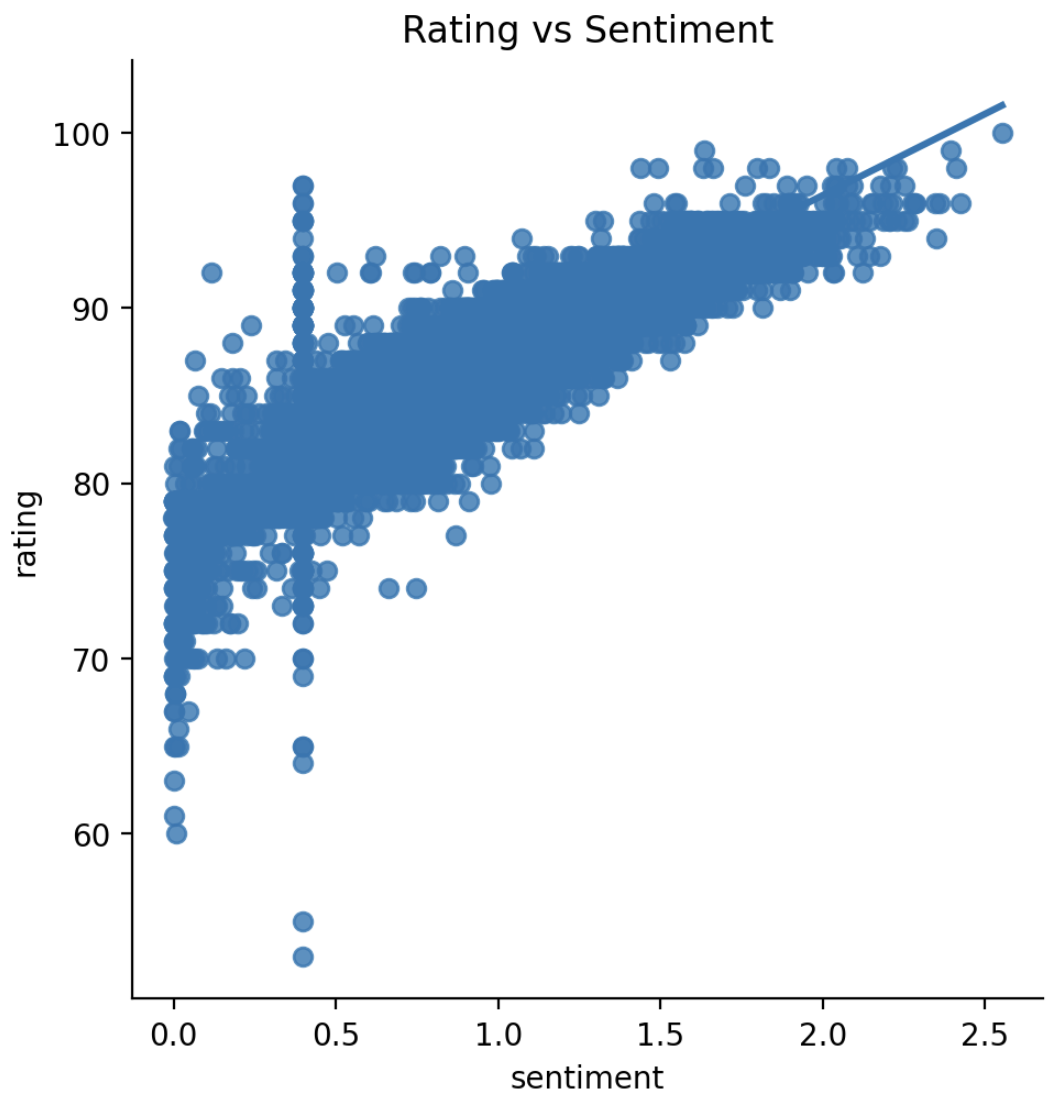
\includegraphics[height=5cm]{sentiment_rating.png}
        \caption{Linear Plots between sentiment and rating}
        \label{fig:sentiment_rating}
    \end{subfigure}
    \hfill
    % Second subfigure
    \begin{subfigure}[b]{0.45\linewidth}
        \centering
        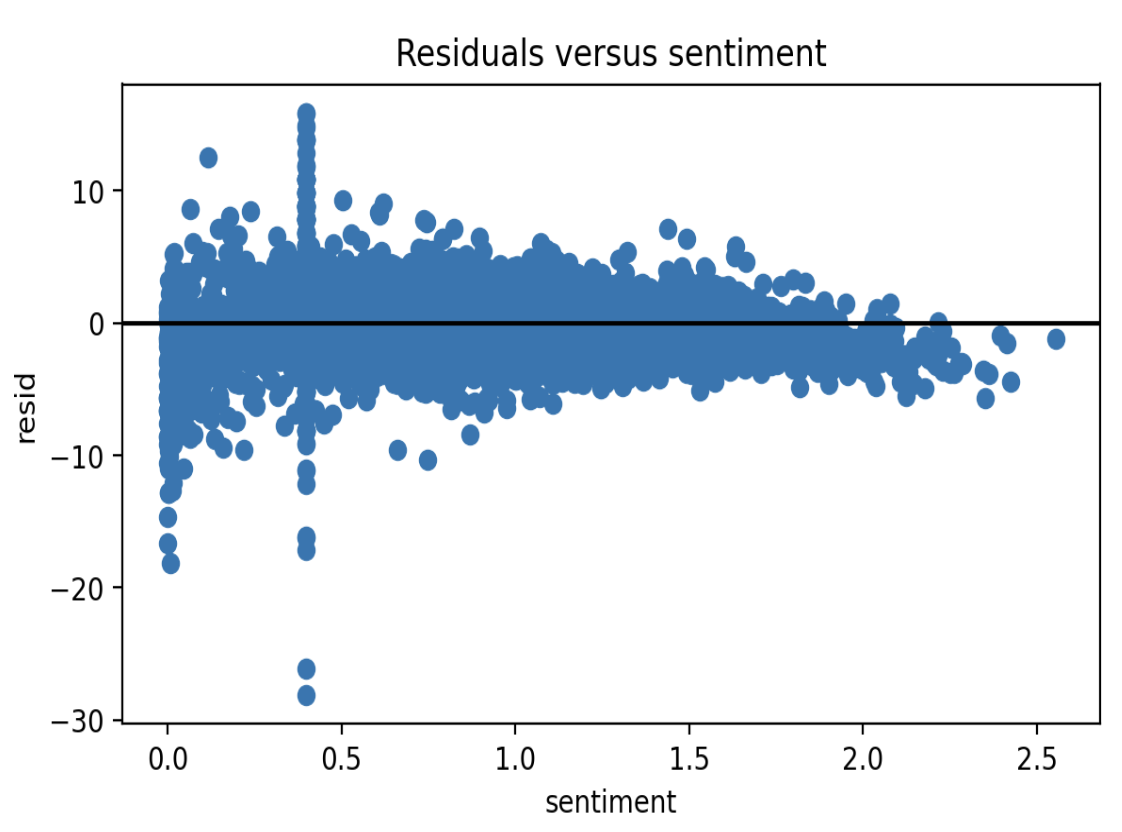
\includegraphics[height=5cm]{residuals.png}
        \caption{Residuals versus sentiment}
        \label{fig:residuals}
    \end{subfigure}
    % Main caption
    \caption{Comparison of model fit and residuals for the regression analysis.}
    \label{fig:side_by_side_equal_height}
\end{figure}
Finally, it is a QQ normal plot to diagnose the linear regression. As we can observe, the beginning curve is below the diagonal line and the tail is above the diagonal line. This heavier tail suggests more extreme values than expected. There are more outliers in rating scores. The linear regression assumption that residuals are normal distribution is slightly compromised but the point estimations are still unbiased. The statistical tests may be inaccurate. One solution to this is to apply robust linear regression to reduce the influence from the outliers. 
\begin{figure}
    \centering
    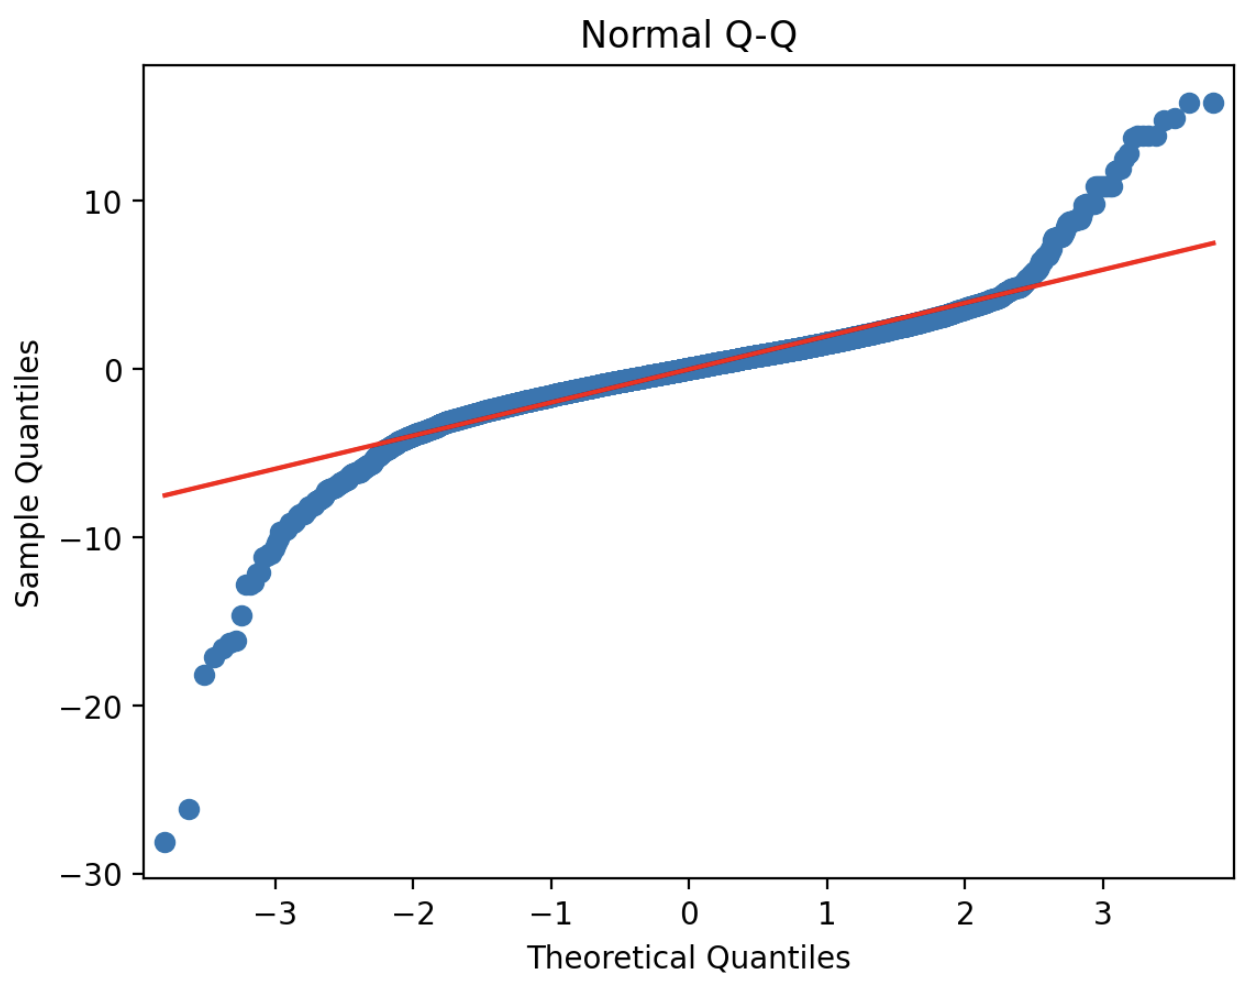
\includegraphics[width=0.3\linewidth]{QQ.png}
    \caption{QQ Normal Plot}
    \label{fig:placeholder}
\end{figure}

The next two plots show the trend of average ratings and average sentiment by year. As we can observe, it is obvious that the average ratings have been increasing over the year from 80 to 90. The similar trend occurs with the average trend of sentiment, increasing from 0.4 to 1.4. This shows that wine reviewers have been rating wines at a higher score over years. 
\begin{figure}[!ht]
    \centering
    % First plot
    \begin{subfigure}[b]{0.45\linewidth}
        \centering
        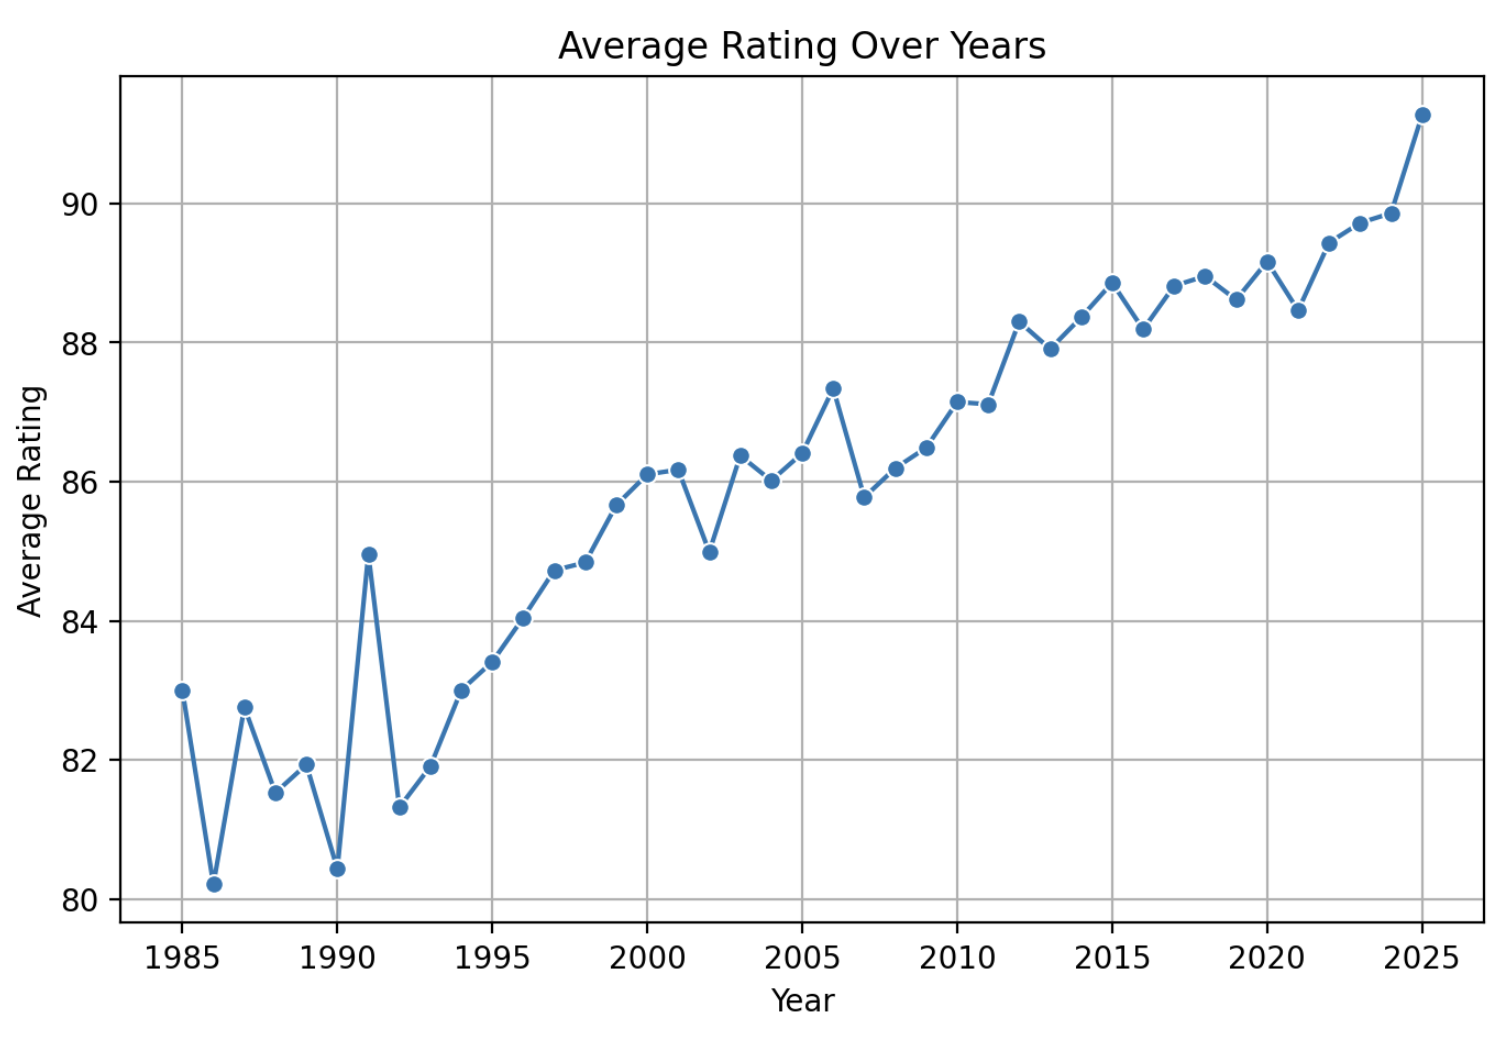
\includegraphics[width=\linewidth]{average_rating.png}
        \caption{Average Rating by year}
        \label{fig:avg_rating}
    \end{subfigure}
    \hfill
    % Second plot
    \begin{subfigure}[b]{0.45\linewidth}
        \centering
        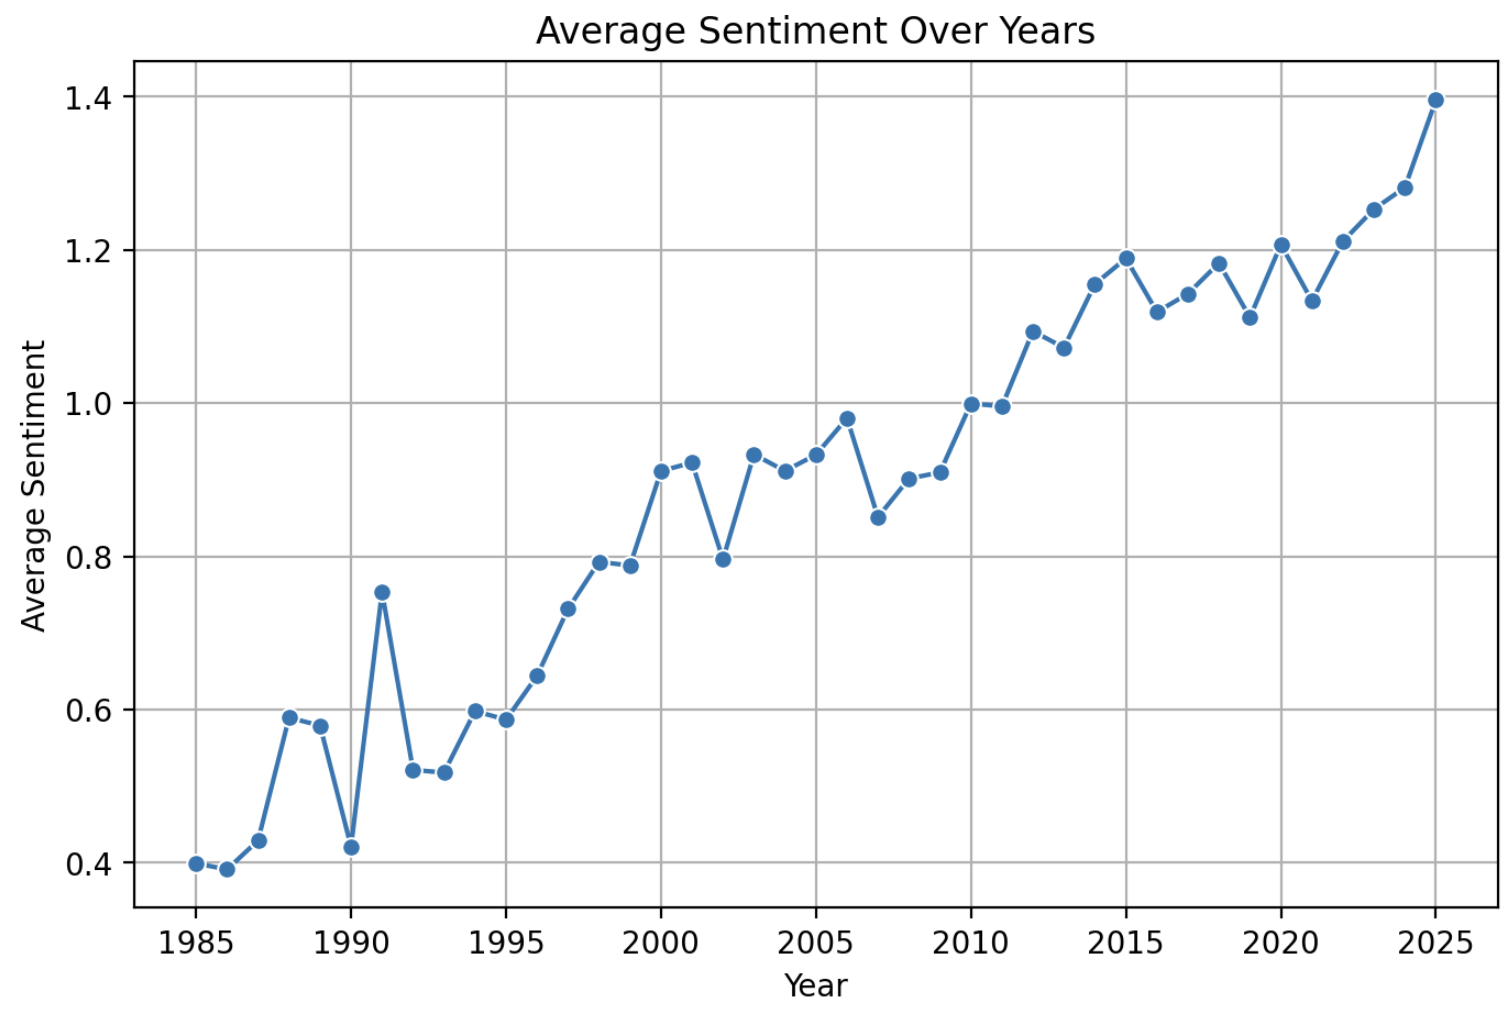
\includegraphics[width=\linewidth]{average_sentiment.png}
        \caption{Average Sentiment by year}
        \label{fig:avg_sentiment}
    \end{subfigure}
    % Main caption
    \caption{Comparison of average rating and sentiment over time.}
    \label{fig:avg_side_by_side}
\end{figure}

\section{Another Linear Regression}
In this section, I used another type of linear regression to measure the impact of year on rating score. I used the year indicator, which is 0 when year is less than 2010 and 1 when year is more than 2010. The variables are one-year indicator, sentiment, and interaction term between year indicator and sentiment. 
$$\text{rating} = \beta_0 + \beta_1 \cdot \text{year\_indicator} + \beta_2 \cdot \text{sentiment} + \beta_3 \cdot \text{year\_indicator:sentiment} + \varepsilon$$
$$E(\text{rating}) = 77.1 + 2.1 \cdot \text{year\_indicator} + 10.0 \cdot \text{sentiment} - 1.8 \cdot \text{year\_indicator:sentiment}$$
The adjusted R squared for this regression is 80.1\% which means this model explains the variations more than the previous simple regression. All three variables are statistically significant. 

\begin{figure}[!ht]
    \centering
    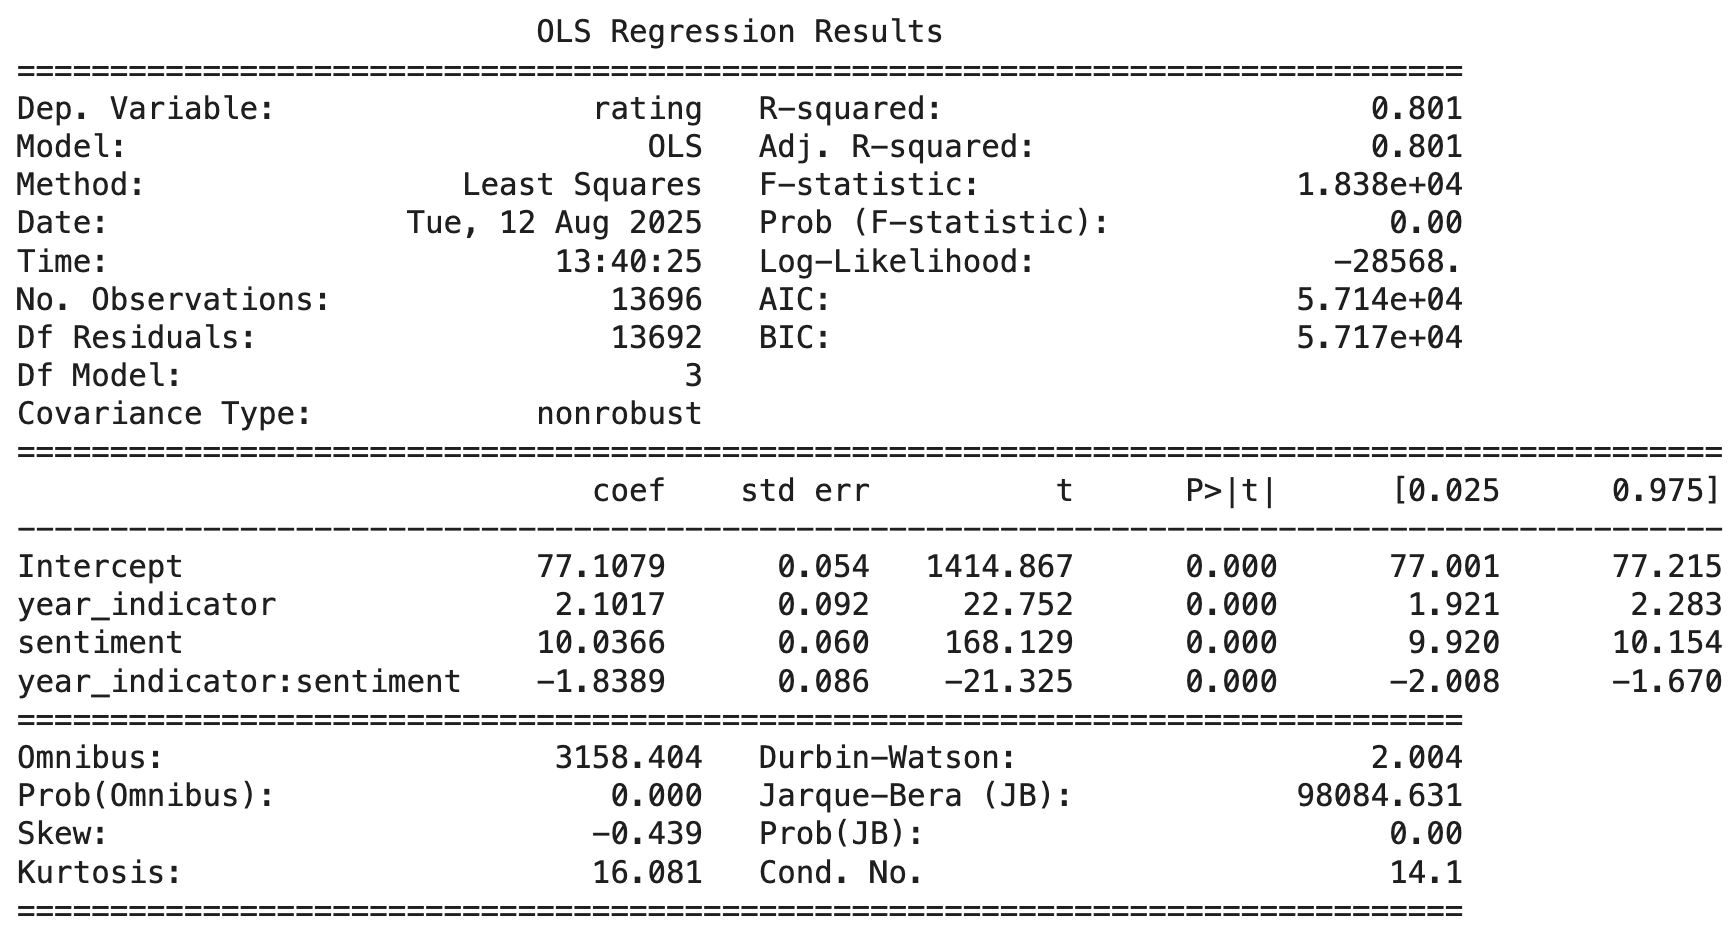
\includegraphics[width=0.6\linewidth]{indicator_regression.png}
    \caption{Summary of this interaction regression}
    \label{fig:placeholder}
\end{figure}
The following two plots are residuals and the QQ normal diagnosis plot. Residuals are evenly scattered across the zero line and the heave tail. shows in the QQ normal plot. 
\begin{figure}[!ht]
    \centering
    % First plot
    \begin{subfigure}[b]{0.45\linewidth}
        \centering
        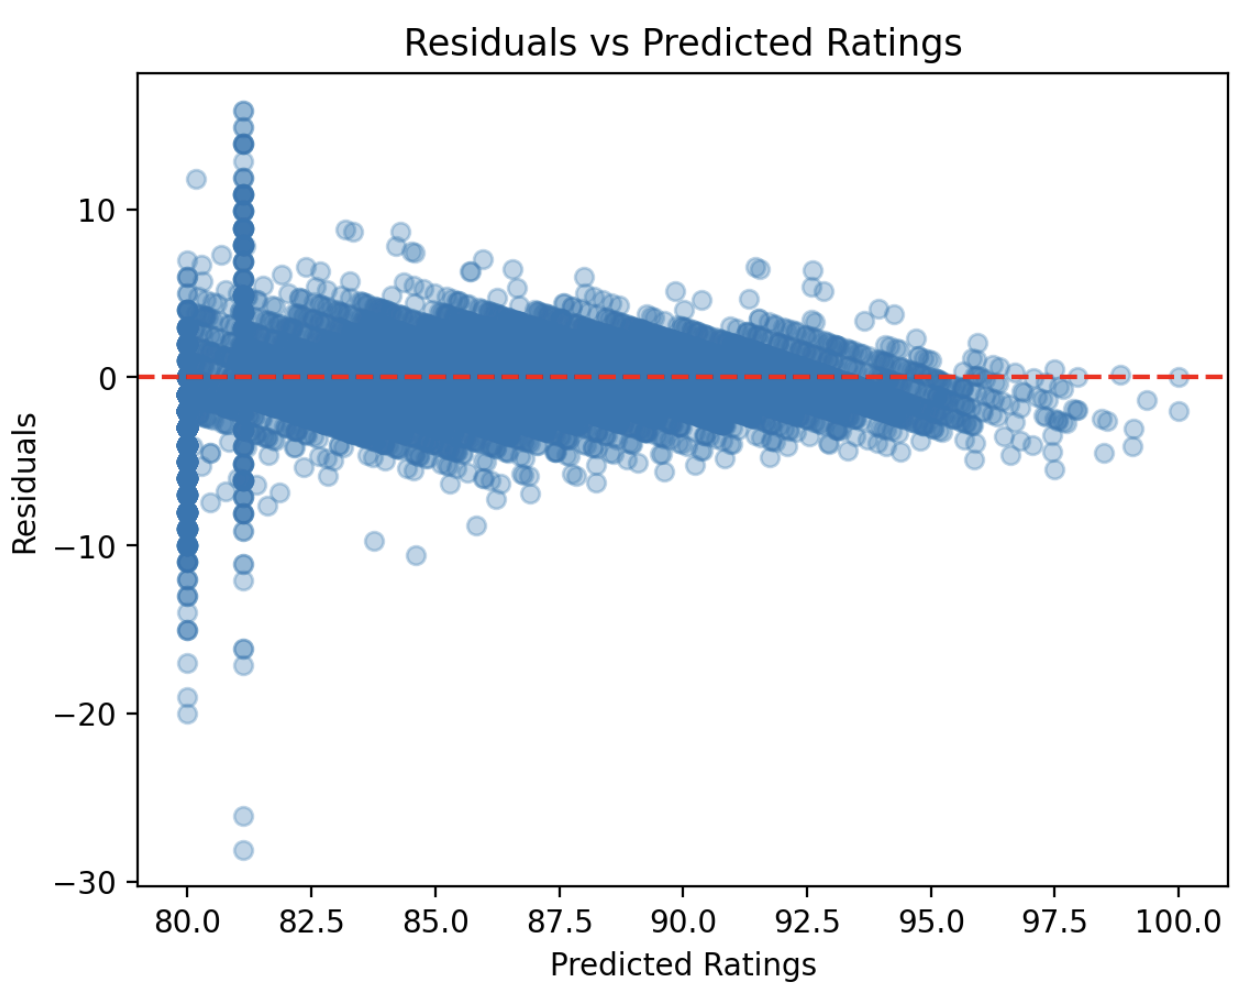
\includegraphics[width=\linewidth]{residuals_interaction.png}
        \caption{Residuals vs. interaction term}
        \label{fig:residuals_interaction}
    \end{subfigure}
    \hfill
    % Second plot
    \begin{subfigure}[b]{0.45\linewidth}
        \centering
        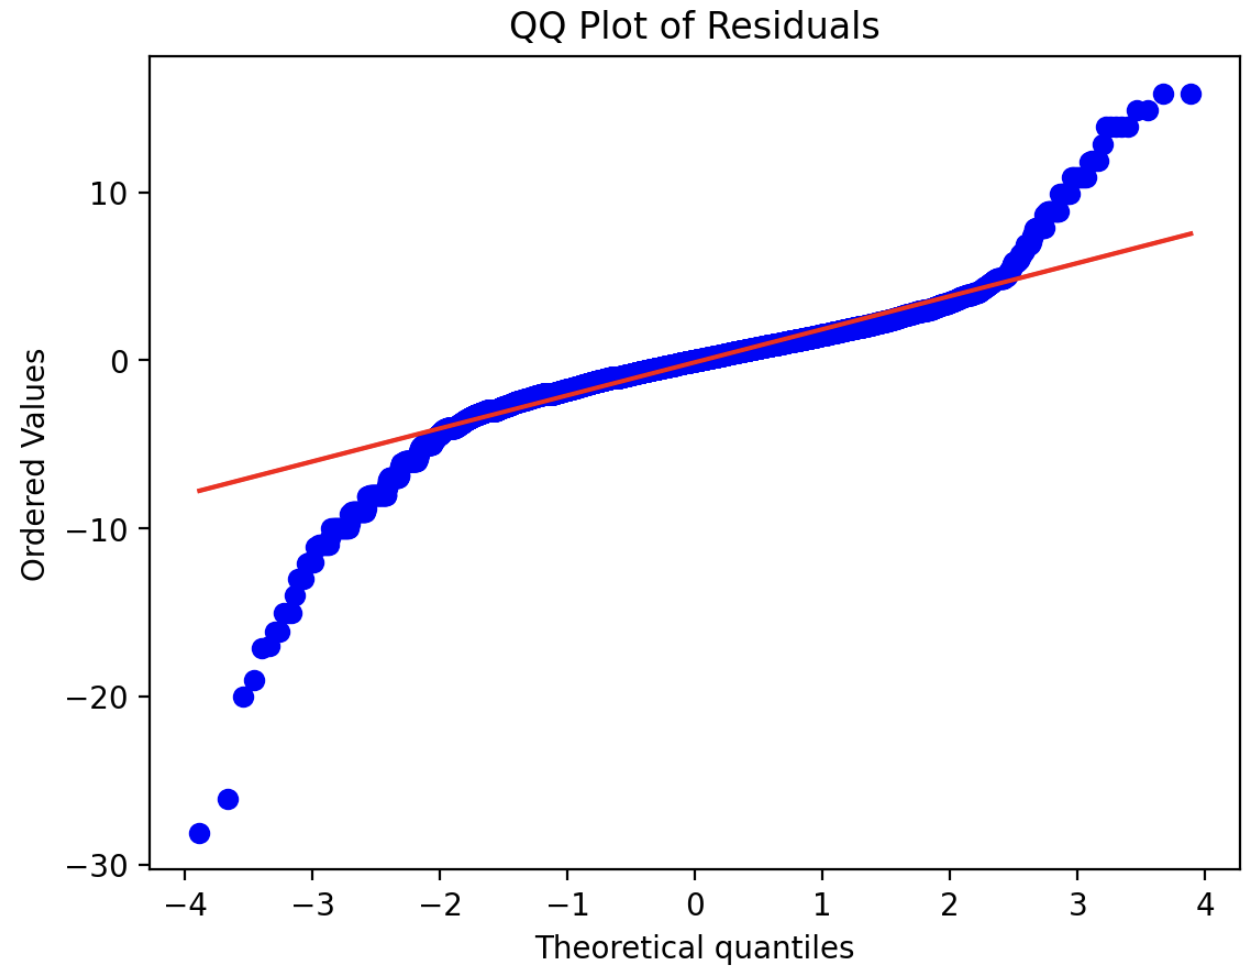
\includegraphics[width=\linewidth]{QQ_interaction.png}
        \caption{QQ plot for interaction model residuals}
        \label{fig:qq_interaction}
    \end{subfigure}
    % Main caption
    \caption{Residual and QQ plots for interaction term model}
    \label{fig:interaction_side_by_side}
\end{figure}

The year indicator coefficient is 2.1 in this regression model, which shows a positive relationship between year indicator and rating. In the first case where the review year is less than 2010, the regression equation becomes into $$E(\text{rating}) = 77.1 + 10.0 \cdot \text{sentiment}$$. This equation shows that every 1 point increase in sentiment will increase the rating by 10. In the second case where the review year is more than 2010, then the regression equation becomes into $$E(\text{rating}) = 79.2 + 8.2\cdot \text{sentiment}$$ The intercept for this regression model is 2.1 higher than the baseline case. This makes sense when the later years would inflate the rating scores. However, the sentiment effect is weaker because every 1 point increase would only increase rating by 8.2 on average. 
The following plot shows the boxplot for two categories. The left box is for cases when review year is less and equal to 2010, and the right box is for cases when review year is larger than 2010. As we can observe, the median value of rating when review year is greater than 2010 is almost same as the upper quartile of rating when review year is less than 2010. 

\begin{figure}
    \centering
    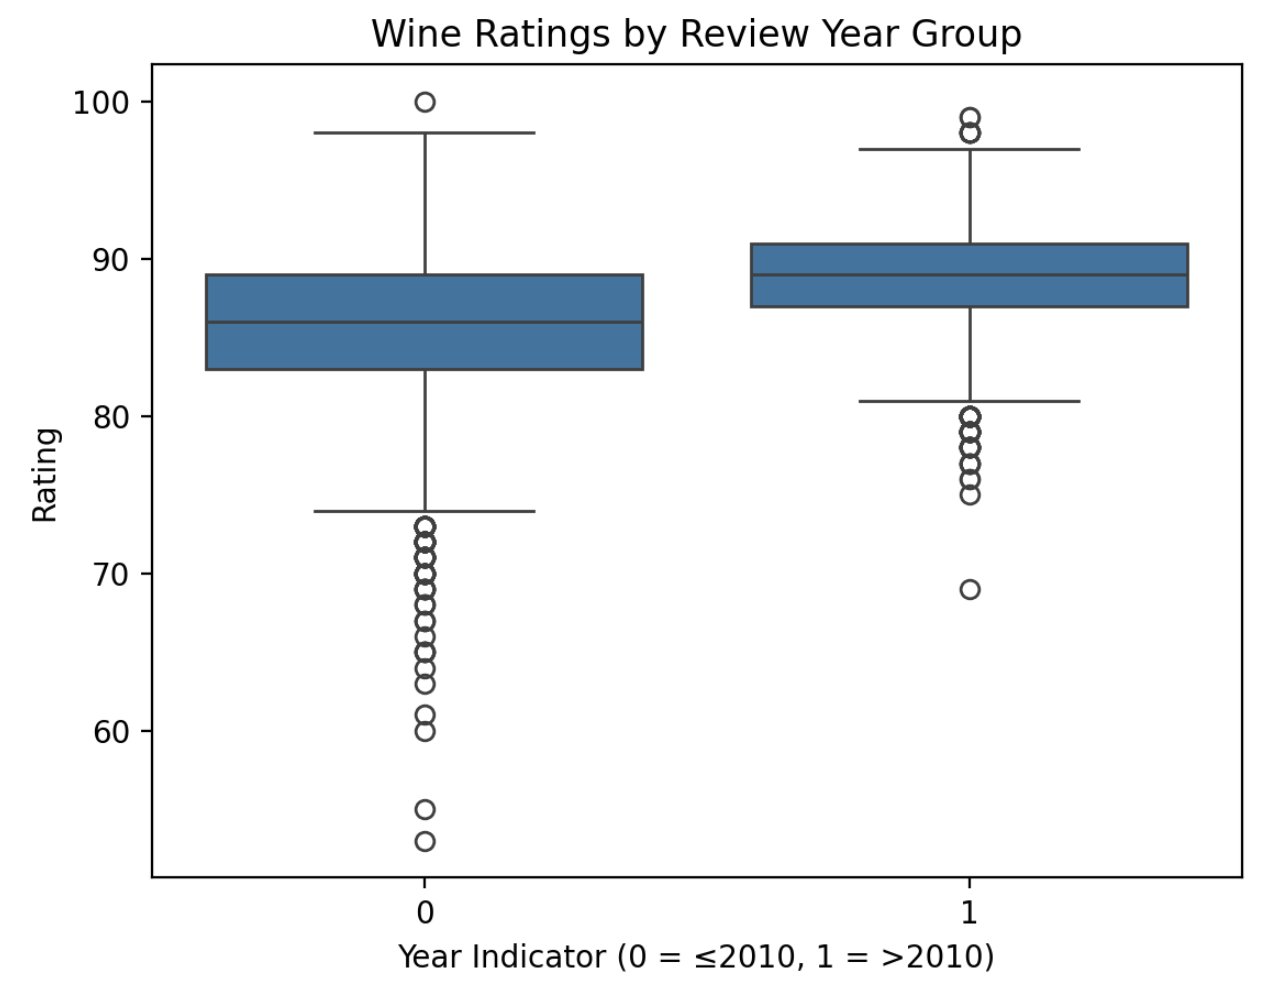
\includegraphics[width=0.5\linewidth]{box.png}
    \caption{Boxplot for two case}
    \label{fig:placeholder}
\end{figure}

\section{Bin Sentiment}
Now I want to visualize the relationship between 'rating' and 'clean\_year' for similar scores of 'sentiment' using scatter plots. I created discrete bins for the 'sentiment' column based on specified intervals. I used the min value of sentiment, 0.5, 1.0, 1.5, 2.0 and max value of sentiment as the intervals to place all sentiment scores into each bin. For each sentiment bin, I created a scatter plot showing the relationship between 'rating' (on the y-axis) and 'clean\_year' (on the x-axis). As we can observe, except for bin 4, in each bin there is a clear up slope trend of rating by year. Bin 3 and Bin 0 have slightly flat trend while Bin 1 and Bin 2 have more clear up slope trend. Bin 4 has down hill trend but we have much less data points, only 69 observations in this bin, so the accuracy of trend is uncertainty. 

\begin{figure}
    \centering
    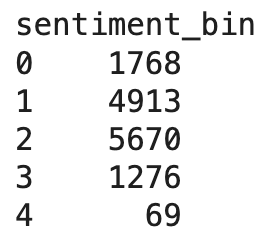
\includegraphics[width=0.3\linewidth]{bins.png}
    \caption{Counts of each bin}
    \label{fig:placeholder}
\end{figure}

\begin{figure}[!ht]
    \centering
    % Row 1
    \begin{subfigure}[b]{0.45\linewidth}
        \centering
        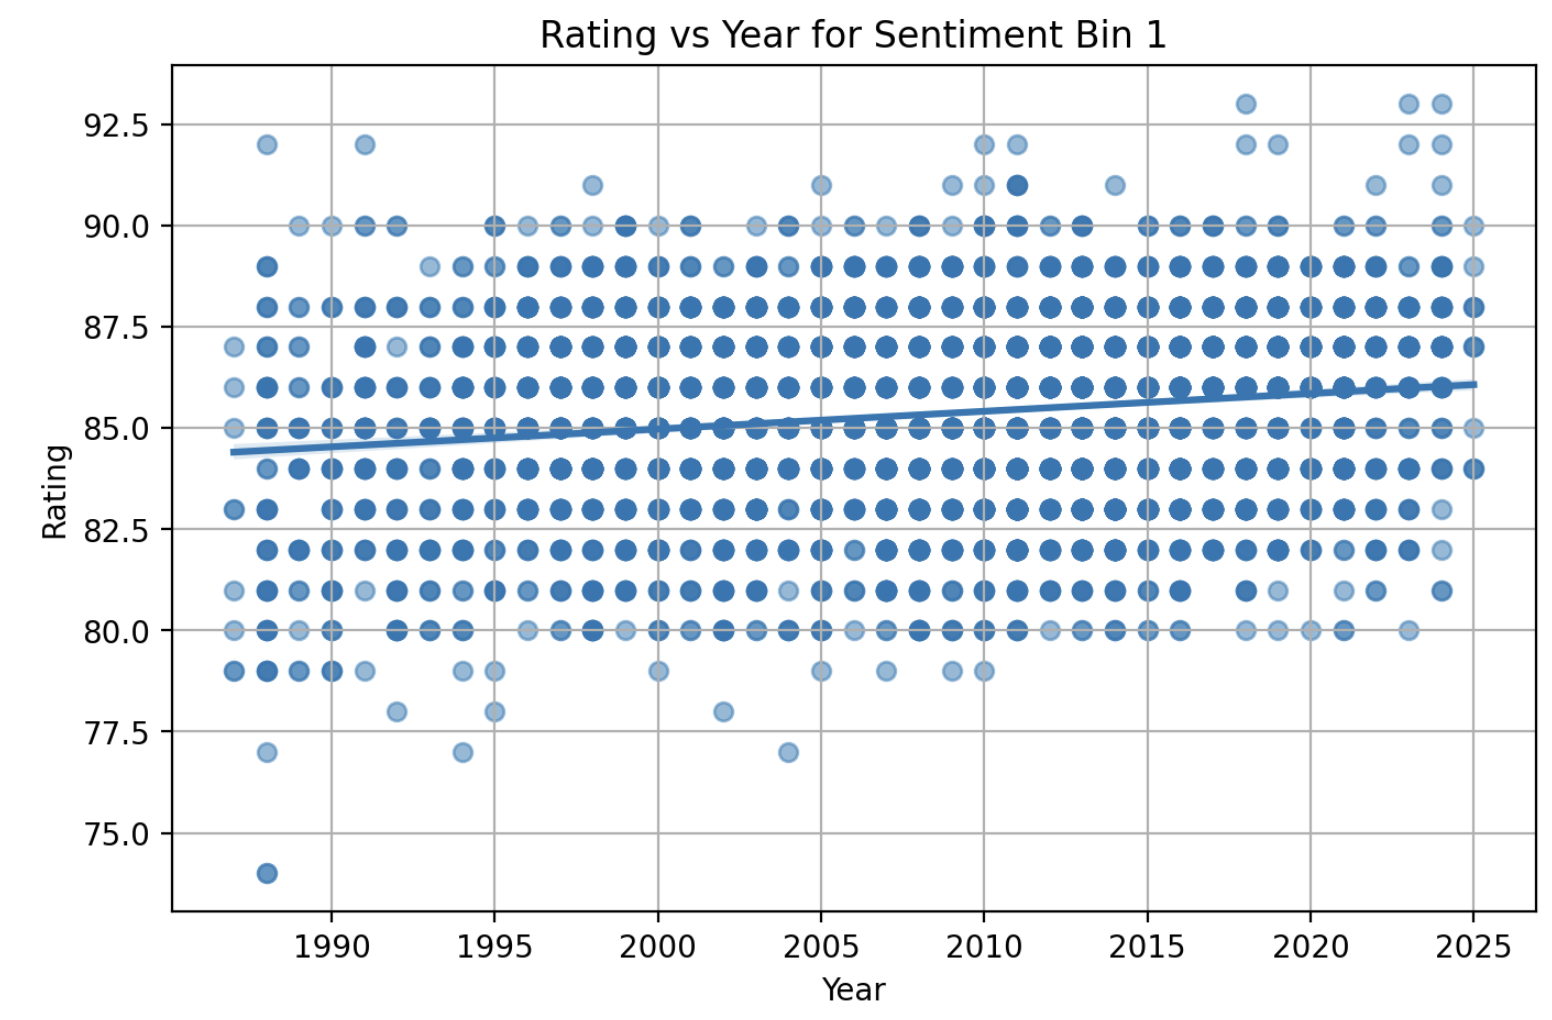
\includegraphics[width=\linewidth]{bin1.png}
        \caption{Bin 1}
        \label{fig:bin1}
    \end{subfigure}
    \hfill
    \begin{subfigure}[b]{0.45\linewidth}
        \centering
        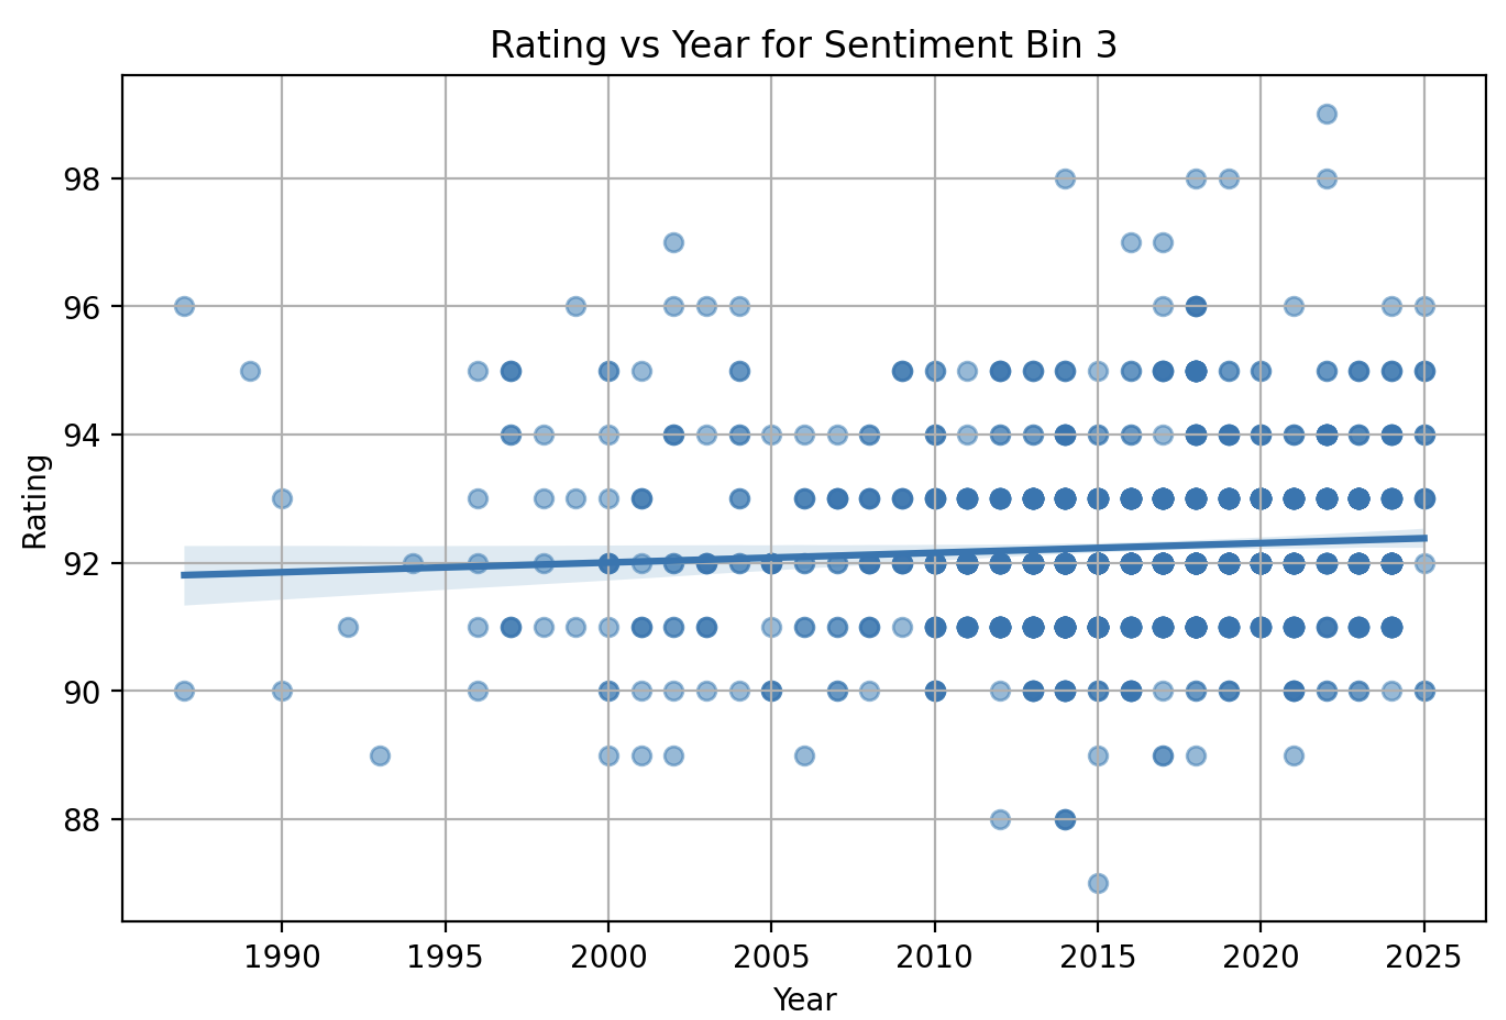
\includegraphics[width=\linewidth]{Bin3.png}
        \caption{Bin 3}
        \label{fig:bin3}
    \end{subfigure}

    \vspace{0.5cm} % Space between rows

    % Row 2
    \begin{subfigure}[b]{0.45\linewidth}
        \centering
        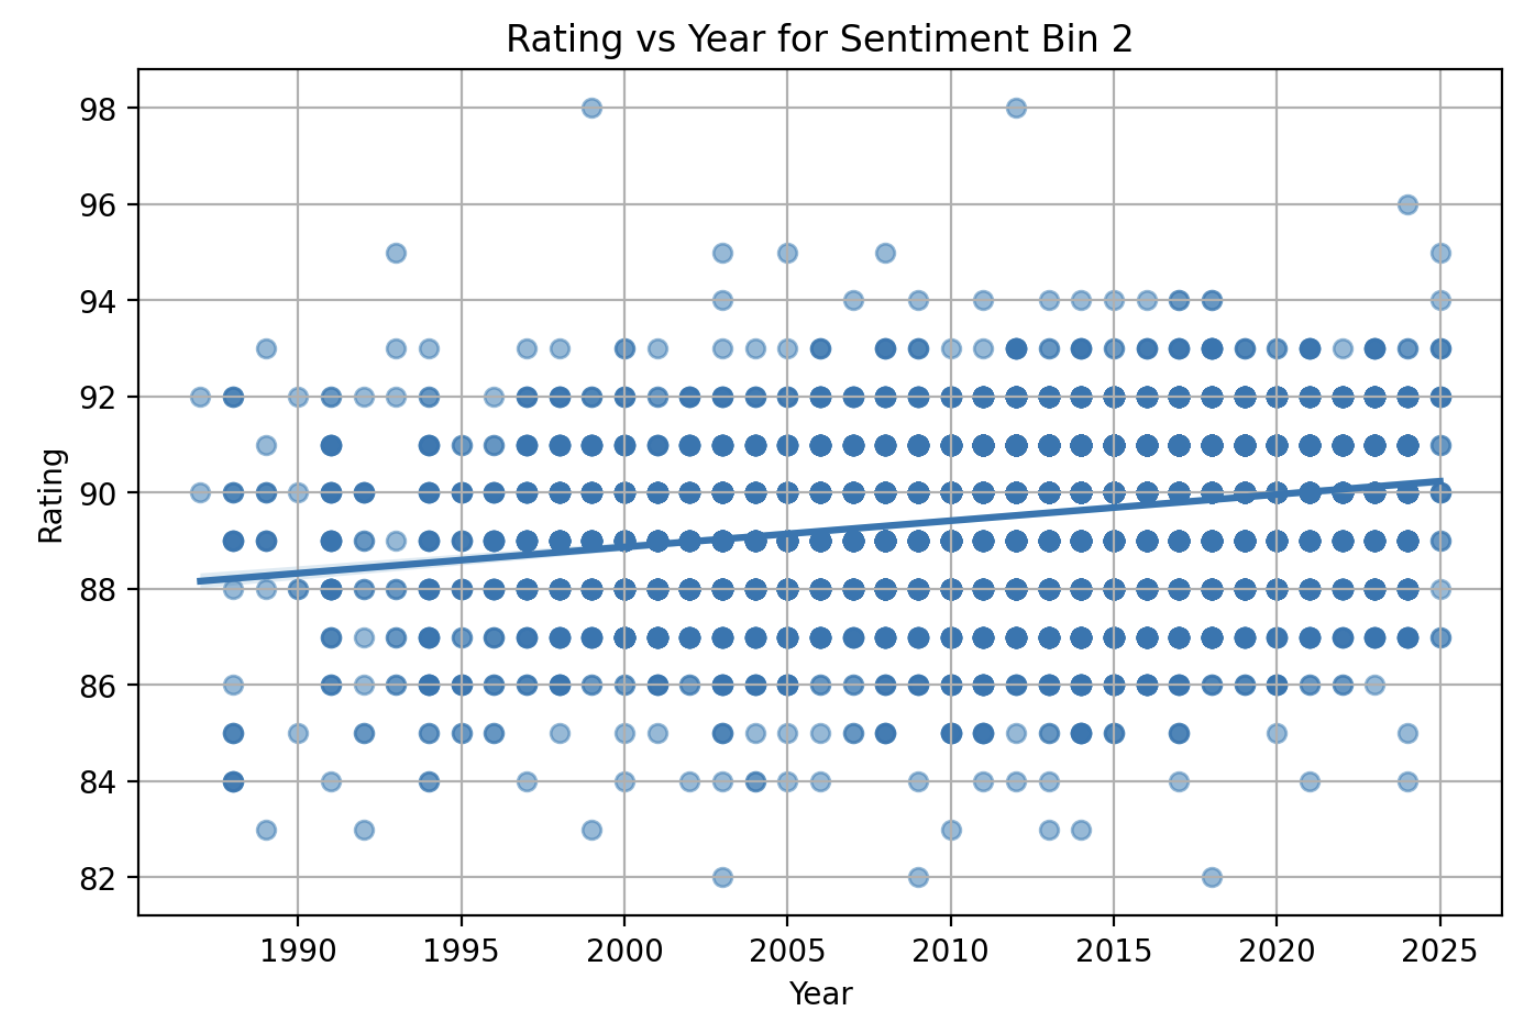
\includegraphics[width=\linewidth]{Bin 2.png}
        \caption{Bin 2}
        \label{fig:bin2}
    \end{subfigure}
    \hfill
    \begin{subfigure}[b]{0.45\linewidth}
        \centering
        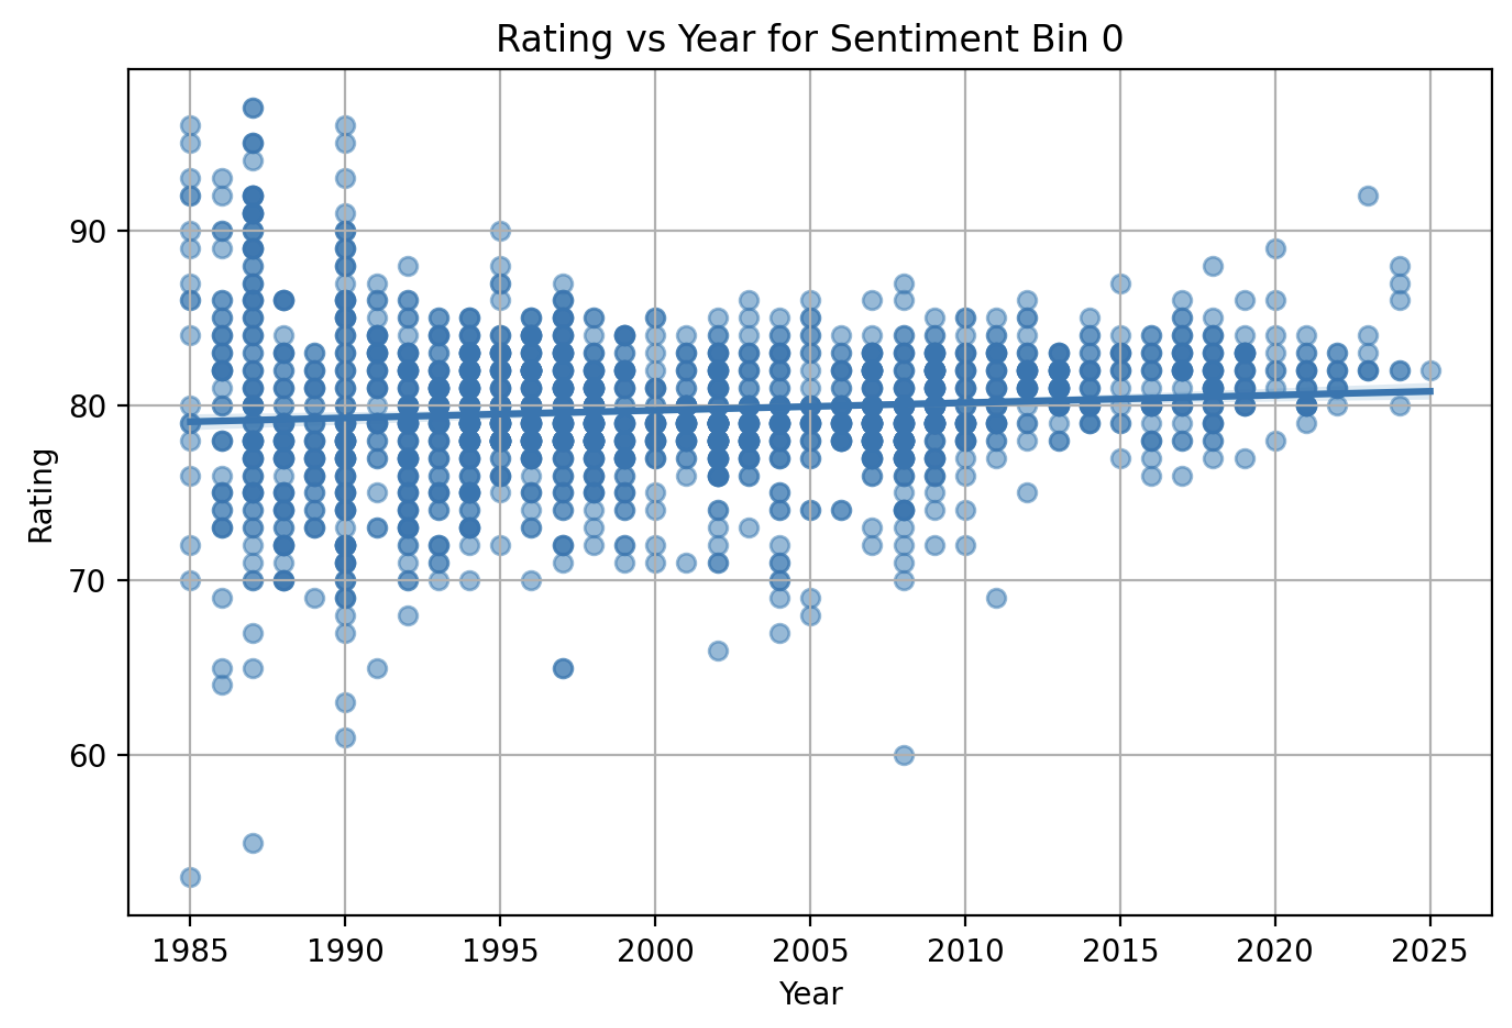
\includegraphics[width=\linewidth]{Bin 0.png}
        \caption{Bin 0}
        \label{fig:bin0}
    \end{subfigure}

    \vspace{0.5cm} % Space between rows

    % Row 3
    \begin{subfigure}[b]{0.45\linewidth}
        \centering
        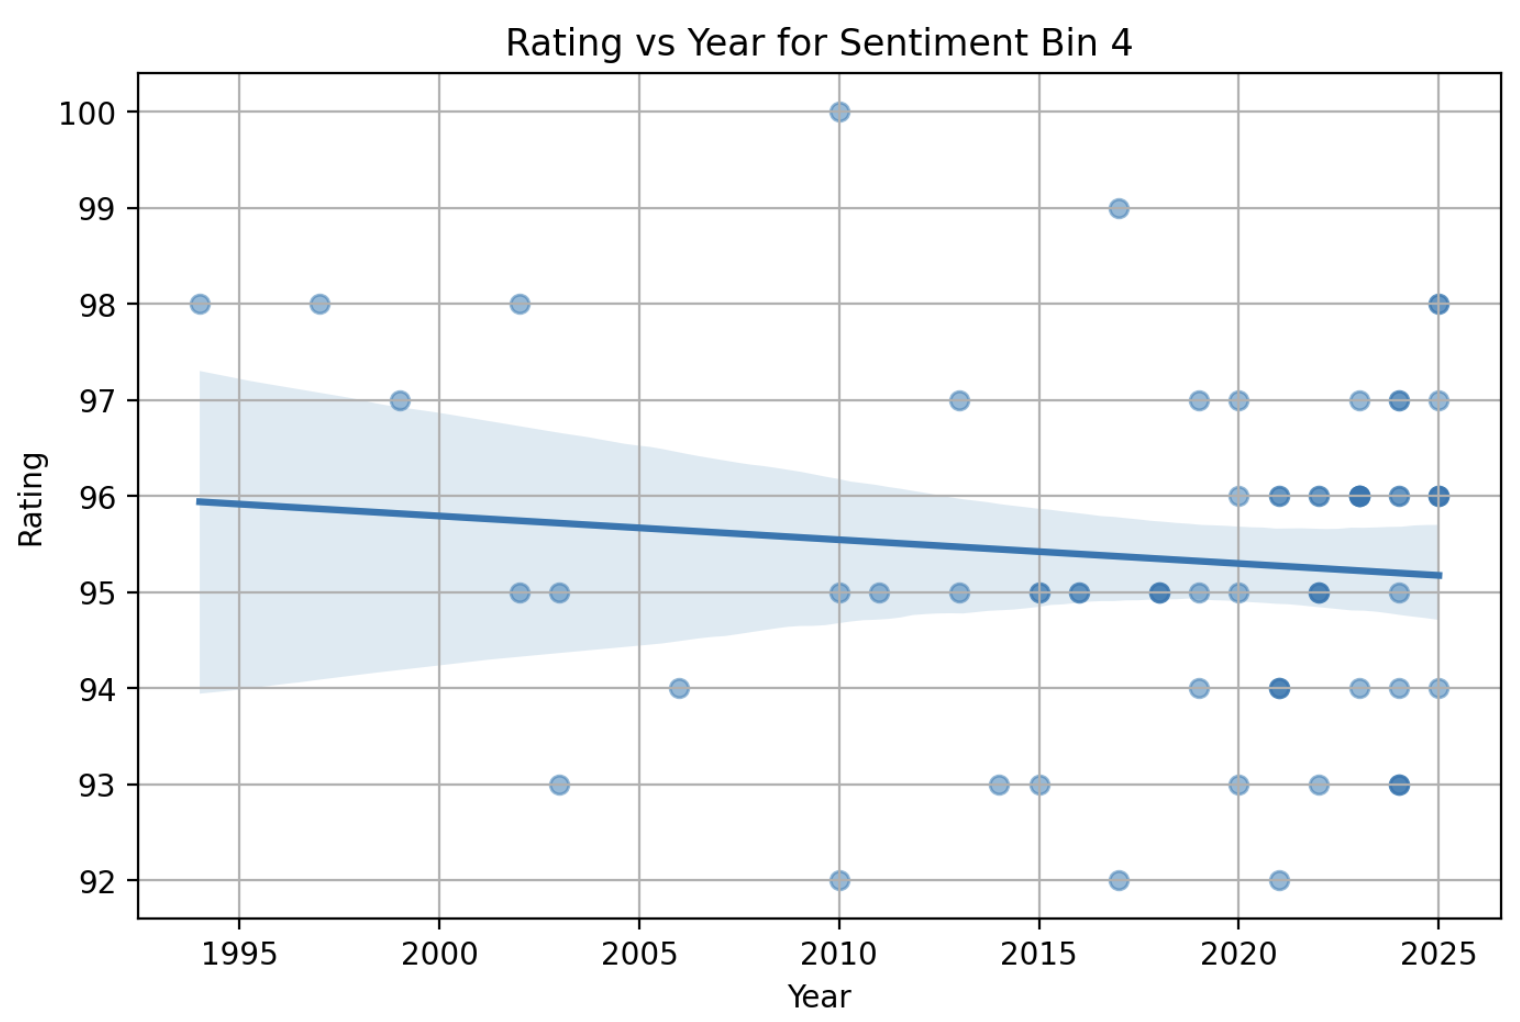
\includegraphics[width=\linewidth]{Bin4.png}
        \caption{Bin 4}
        \label{fig:bin4}
    \end{subfigure}

    \caption{Comparison of ratings and sentiments across different bins}
    \label{fig:bins_side_by_side}
\end{figure}


\end{document}
